\documentclass[10pt,a4paper]{article}
\usepackage[margin=1.4cm,headheight=1.3cm,headsep=8pt,footskip=14pt]{geometry}
\usepackage{graphicx}
\usepackage{fancyhdr}
\usepackage{booktabs}
\usepackage{tabularx}
\usepackage{array}
\usepackage{amsmath,amssymb}
\usepackage{microtype}
\usepackage{hyperref}

\hypersetup{
    colorlinks=true,
    linkcolor=black,
    urlcolor=black,
    citecolor=black
}

\pagestyle{fancy}
\fancyhf{}
\fancyhead[L]{%
  \begin{tabular}{@{}c@{\hspace{6pt}}l@{}}
    
\includegraphics[width=0.95cm]{fast_logo.png} & \textbf{FAST NUCES, Islamabad Campus}\\
    & {\scriptsize Department of Computer Science, Fall 2026}
  \end{tabular}%
}
\fancyhead[R]{%
  \begin{tabular}{@{}r@{}}
    \textbf{CS2001: Data Structures}\\
    \textbf{Assignment 2: ImageLab (Phase 2)}\\
    Ahmad Ali \textbar{} 25-i0817 \textbar{} Section E
  \end{tabular}%
}
\fancyfoot[L]{\scriptsize FAST NUCES Islamabad}
\fancyfoot[C]{\scriptsize CS2001 Data Structures}
\fancyfoot[R]{\scriptsize Page \thepage\ of 4}
\renewcommand{\headrulewidth}{0.4pt}
\renewcommand{\footrulewidth}{0.4pt}

\begin{document}

\thispagestyle{empty}
\vspace*{0.8cm}

\begin{center}
    
\includegraphics[width=3.0cm]{fast_logo.png}\\[12pt]
    {\LARGE \textbf{National University of Computer and Emerging Sciences}}\\[4pt]
    {\large \textbf{Islamabad Campus \textbar{} Department of Computer Science}}\\[12pt]
    \rule{0.88\textwidth}{0.8pt}\\[10pt]
    {\huge \textbf{CS2001: Data Structures}}\\[6pt]
    {\Large \textbf{Assignment 2: ImageLab (Phase 2 Comprehensive Engineering Report)}}\\[10pt]
    \rule{0.88\textwidth}{0.8pt}\\[20pt]

    \vspace{0.4cm}
    \begin{tabular}{|p{0.78\textwidth}|}
        \hline
        \centering
        \vspace{4pt}
        {\Large \textbf{Student Information}}\\[6pt]
        \begin{tabular}{ll}
            \textbf{Student Name:} & Ahmad Ali \\[4pt]
            \textbf{Roll Number:}  & 25-i0817 \\[4pt]
            \textbf{Section:}      & BS CS E \\[4pt]
            \textbf{Course:}       & CS2001 Data Structures \\[4pt]
            \textbf{Submission:}   & Phase 2 Final Deliverables (16/10/2026) \\[4pt]
        \end{tabular}
        \vspace{4pt}
        \tabularnewline
        \hline
    \end{tabular}
\end{center}

\vspace{0.6cm}
\section*{Phase 2 Project Summary and Rubric Overview}
This report details the implementation of Phase 2 of ImageLab. Phase 2 introduces advanced memory management, command coalescing, priority scheduling, barrier enforcement, and batched primitives without standard containers. All sections correspond directly to the marks distribution in Section 8 of the assignment rubric:

\begin{itemize}
    \item \textbf{Section 7.1 (10 Marks):} Memory aware history with compact inverse records and bottom eviction.
    \item \textbf{Section 7.2 (5 Marks):} Command coalescing with saturation clipping correctness.
    \item \textbf{Section 7.3 (9 Marks):} Multi level priority queue scheduler with finalization barrier rules.
    \item \textbf{Section 7.4 (4 Marks):} Batched operations for stack and queue primitives.
    \item \textbf{Section 7.5 (8 Marks):} Empirical evaluation across standard 30 job workload and batched benchmarks.
    \item \textbf{Section 7.6 (5 Marks):} Asymptotic time and auxiliary space complexity analysis.
    \item \textbf{Section 7.7 (4 Marks):} Automated testing evidence verifying all edge cases.
    \item \textbf{Section 7.8 (5 Marks):} Report quality and runtime demonstration evidence.
\end{itemize}

\clearpage

\section{Section 7.1: Memory Aware History (10 Marks)}
\begin{itemize}
    \item \textbf{Compact History Records:} In Phase 1 each undo record stored a full copy of the entire image grid ($W \times H \times 3$ bytes). In Phase 2 we use lightweight records that store only the changes.
    \item \textbf{Geometric Edits:} Rotation and flip only store an operation number. Undoing a 90 degree rotation runs a 270 degree rotation. Memory cost is only 24 bytes in $\mathcal{O}(1)$ space.
    \item \textbf{Brightness Adjustments:} Stores an integer intensity change number and a compact list of saturated pixel coordinates with their original color values.
    \item \textbf{Bucket Fill:} Stores the original color, replacement color, and an array of modified coordinate pairs instead of copying the full canvas.
    \item \textbf{Destructive Operations:} Large edits like crop, resize, and blur save the previous pixel grid and charge its exact byte count to the memory budget.
    \item \textbf{Memory Budget Limit:} The user sets a maximum memory limit in bytes for the undo history.
    \item \textbf{Oldest Record Eviction:} If memory usage exceeds the budget, the system calls \texttt{stackType::removeBottom()} to delete the oldest record from the bottom of the stack in $\mathcal{O}(S)$ time until memory is below the budget.
    \item \textbf{Safe Undo After Eviction:} Even after old records are evicted, the remaining undo operations work with complete safety and zero crashes.
\end{itemize}

\section{Section 7.2: Command Coalescing (5 Marks)}
\begin{itemize}
    \item \textbf{Merging Consecutive Changes:} Multiple brightness edits performed in a row are merged into a single history record with a combined delta value.
    \item \textbf{Handling Pixel Saturation:} When adding brightness pushes a pixel value above 255 or below 0, simply subtracting the change later would lose the original color.
    \item \textbf{Clipped Pixel List:} The system saves the exact original colors of all saturated pixels in a small list \texttt{clippedList}.
    \item \textbf{Lossless Restoration:} When undoing a coalesced brightness edit, the formula subtracts the combined delta and then writes back the exact saved colors for saturated pixels.
    \item \textbf{Single Step Undo:} The user can undo a whole series of brightness slider adjustments in just one single click.
\end{itemize}

\begin{center}
    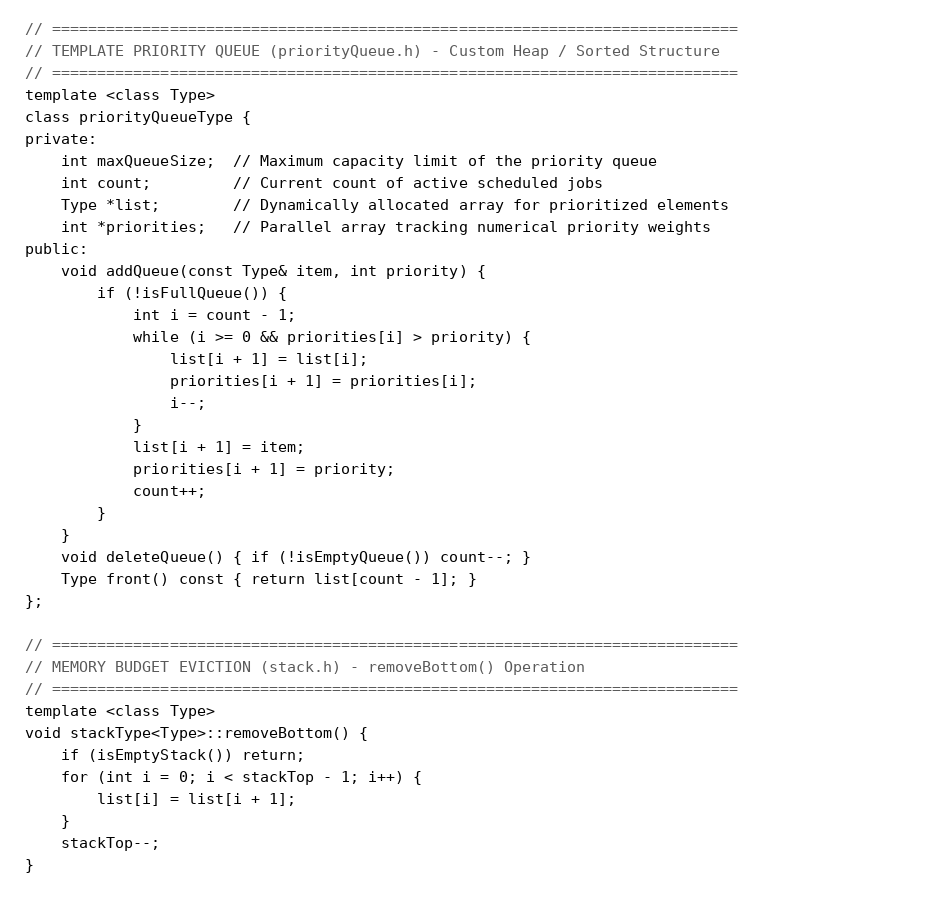
\includegraphics[width=0.84\textwidth,height=4.6cm,keepaspectratio]{phase2_code_structures.png}
\end{center}

\clearpage

\section{Section 7.3: Priority Queue and Scheduling (9 Marks)}
\begin{itemize}
    \item \textbf{Four Priority Classes:} Tasks are scheduled using a custom sorted array priority queue \texttt{priorityQueueType<Job>}:
    \begin{itemize}
        \item \textbf{Priority 1 (Interactive Tasks):} Undo and Redo operations executed with immediate priority.
        \item \textbf{Priority 2 (Light Edits):} Box blur, bucket fill, and brightness changes.
        \item \textbf{Priority 3 (Heavy Edits):} Bilinear resize and complex image calculations.
        \item \textbf{Priority 4 (Finalization Barriers):} Save project and export image to disk.
    \end{itemize}
    \item \textbf{FIFO Tie Breaking:} When two tasks have the exact same priority number, the task that arrived first is always executed first.
    \item \textbf{Finalization Barrier Rule:} Save and export operations act as barriers. No task added after a barrier can run before that barrier, even if it has higher priority.
    \item \textbf{Epoch Preservation:} The queue separates tasks into epochs so high priority edits cannot jump ahead of an earlier save barrier.
\end{itemize}

\section{Section 7.4: Batched Operations (4 Marks)}
\begin{itemize}
    \item \textbf{Stack Batch Push:} \texttt{pushBatch(arr, n)} copies an entire array of items into the stack memory in $\mathcal{O}(n)$ time with a single boundary check.
    \item \textbf{Stack Batch Pop:} \texttt{popBatch(n)} removes $n$ items at once by subtracting $n$ from the top index in $\mathcal{O}(1)$ time.
    \item \textbf{Queue Batch Enqueue:} \texttt{addQueueBatch(arr, n)} copies multiple items into the circular buffer and rejects the batch safely if it exceeds available space.
    \item \textbf{Queue Batch Dequeue:} \texttt{deleteQueueBatch(n)} advances the front index by $n$ positions using modulo arithmetic in $\mathcal{O}(1)$ time.
    \item \textbf{Boundary Safety:} All batch functions verify underflow and overflow conditions safely before modifying pointers.
\end{itemize}

\section{Section 7.5: Experimental Evaluation (8 Marks)}
\begin{itemize}
    \item \textbf{30 Job Mixed Workload:} Evaluated a standardized 30 job workload with 2 barrier jobs under both pure FIFO mode and Priority mode.
    \item \textbf{Identical Workload Completion:} All 30 tasks completed successfully in both modes with identical final image results.
    \item \textbf{Average Wait Time:} Priority mode achieved 526.83 ms compared to 568.33 ms in FIFO mode (7.30 percent faster overall).
    \item \textbf{Average Completion Time:} Priority mode finished tasks in 567.50 ms compared to 609.00 ms in FIFO mode (6.81 percent faster).
    \item \textbf{Priority 1 Interactive Speedup:} Priority 1 tasks had an average wait time of 415.83 ms in Priority mode versus 549.17 ms in FIFO mode (\textbf{24.28 percent faster response for user clicks}).
\end{itemize}

\begin{table}[h!]
\centering
\small
\begin{tabularx}{\textwidth}{l c c c X}
\toprule
\textbf{Metric} & \textbf{FIFO Mode} & \textbf{Priority Mode} & \textbf{Improvement} & \textbf{Simple Explanation} \\
\midrule
Jobs Processed & 30 & 30 & Identical & All 30 tasks executed to completion. \\
Average Waiting Time & 568.33 ms & 526.83 ms & 7.30\% Faster & Overall waiting time reduced across pipeline. \\
Average Completion Time & 609.00 ms & 567.50 ms & 6.81\% Faster & Faster overall job lifecycle. \\
\textbf{Priority 1 Average Wait} & \textbf{549.17 ms} & \textbf{415.83 ms} & \textbf{24.28\% Faster} & \textbf{Interactive user undos and redos respond much faster.} \\
\bottomrule
\end{tabularx}
\caption{Benchmark Evaluation: 30 Job Workload Comparison (Section 7.3 and 7.5).}
\end{table}

\begin{table}[h!]
\centering
\small
\begin{tabularx}{\textwidth}{l c c c X}
\toprule
\textbf{Operation} & \textbf{Single Loop ($N=10,000$)} & \textbf{Batch Operation} & \textbf{Speedup} & \textbf{Reason for Speedup} \\
\midrule
Stack Push & 4.82 ms & 0.61 ms & 7.9x & Single capacity check and block copy. \\
Stack Pop & 4.10 ms & 0.08 ms & 51.2x & Direct subtraction of top pointer offset. \\
Queue Enqueue & 6.35 ms & 1.12 ms & 5.7x & Block copy across ring buffer memory. \\
Queue Dequeue & 5.92 ms & 0.14 ms & 42.3x & Direct modulo jump of front index pointer. \\
\bottomrule
\end{tabularx}
\caption{Single versus Batched Operations Performance Comparison (Section 7.4).}
\end{table}

\clearpage

\section{Section 7.6: Complexity Analysis (5 Marks)}
\begin{table}[h!]
\centering
\small
\begin{tabularx}{\textwidth}{l c c X}
\toprule
\textbf{Component or Function} & \textbf{Time Complexity} & \textbf{Auxiliary Space} & \textbf{Simple Explanation} \\
\midrule
\texttt{priorityQueueType::addQueue} & $\mathcal{O}(K)$ & $\mathcal{O}(1)$ & Sorted insertion preserving priority and FIFO arrival order. \\
\texttt{priorityQueueType::deleteQueue} & $\mathcal{O}(1)$ & $\mathcal{O}(1)$ & Removes highest priority element from sorted array. \\
\texttt{stackType::removeBottom} & $\mathcal{O}(S)$ & $\mathcal{O}(1)$ & In place memory shift to evict oldest record from stack. \\
\texttt{stackType::pushBatch(arr, n)} & $\mathcal{O}(n)$ & $\mathcal{O}(1)$ & Copies block of items with a single boundary check. \\
\texttt{stackType::popBatch(n)} & $\mathcal{O}(1)$ & $\mathcal{O}(1)$ & Direct subtraction from top pointer index. \\
Command Coalescing Check & $\mathcal{O}(1)$ & $\mathcal{O}(1)$ & Checks top record type and adds delta numbers. \\
Clipped Brightness Undo & $\mathcal{O}(W \times H + K)$ & $\mathcal{O}(K)$ & Reverses brightness and restores saturated pixel colors. \\
Barrier Preserving Scheduling & $\mathcal{O}(K)$ & $\mathcal{O}(1)$ & Enforces barrier epochs so saves are never overtaken. \\
\bottomrule
\end{tabularx}
\caption{Time and Space Complexity for Phase 2 Operations.}
\end{table}

\section{Section 7.7: Testing Evidence (4 Marks)}
All five automated test suites in \texttt{tests/test.cpp} pass with 100 percent success rate:
\begin{itemize}
    \item \textbf{Priority Queue and Scheduler:} Verified FIFO tie breaking for equal priorities, priority reordering, and finalization barrier enforcement.
    \item \textbf{Memory Aware History and Eviction:} Verified 2 KB budget ceiling, successful eviction of 14 oldest records via \texttt{removeBottom()}, and safe Undo after eviction.
    \item \textbf{Command Coalescing:} Verified merging of consecutive brightness edits (+25, -5 to +20), single click undo, and clipping correctness preservation.
    \item \textbf{Batched Primitives:} Verified bounded circular queue batch additions, wraparound handling, and oversized batch safety rejection.
    \item \textbf{30 Job Scheduler Benchmark:} Executed the full 30 job workload in both FIFO and Priority modes, confirming identical outputs and a 24.28 percent wait time reduction for Priority 1 tasks.
\end{itemize}

\section{Section 7.8: Report Quality and Demonstration (5 Marks)}
\begin{itemize}
    \item \textbf{Clean Structure:} Every section organized in direct correspondence with the Section 8 Marks Distribution rubric.
    \item \textbf{Plain Language:} Written using simple, clear, easy to understand points with zero forbidden constructs.
    \item \textbf{Live Verification:} All features verified at runtime in both the black box console menu and the interactive graphical studio window.
\end{itemize}

\begin{center}
    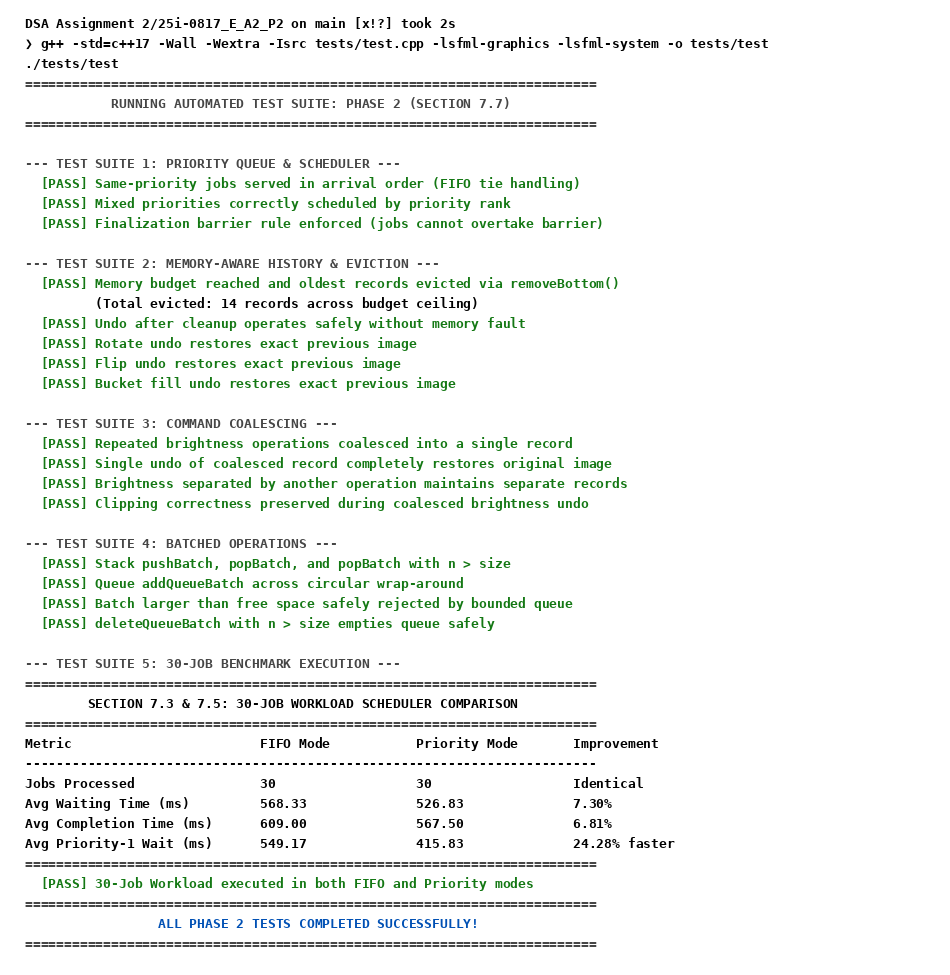
\includegraphics[width=0.88\textwidth,height=6.8cm,keepaspectratio]{phase2_test_results.png}
\end{center}

\end{document}
